\usetikzlibrary{shapes,positioning,decorations.pathmorphing}

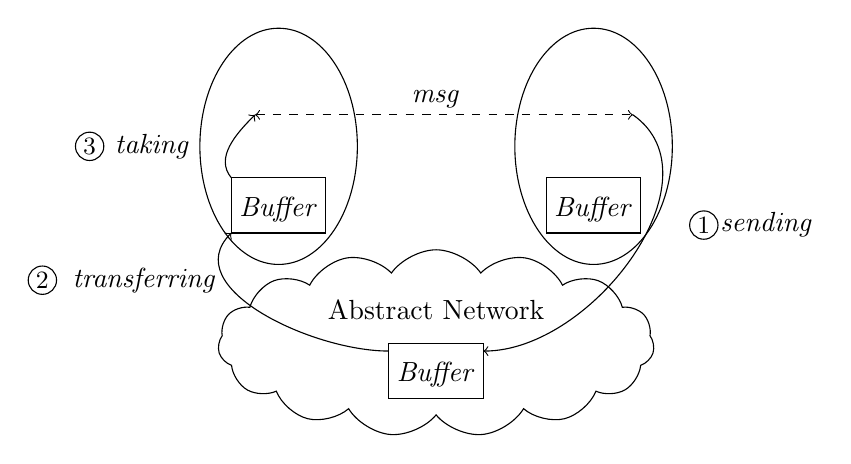
\begin{tikzpicture}%[arrow/.style = {draw=#1,-{Stealth[]}, shorten >=1mm, shorten <=1mm}]

\draw  (0,2.5) ellipse (1 and 1.5);
\draw  (-0.6,2.1) rectangle (0.6,1.4);
\node at (0,1.7) {$\it Buffer$};

\draw  (4,2.5) ellipse (1 and 1.5);
\draw  (3.4,2.1) rectangle (4.6,1.4);
\node at (4,1.7) {$\it Buffer$};

\draw[<->,dashed] (-0.3,2.9) -- (4.5,2.9) ;
\node at (2,3.1) {$\it msg$};

 \node[cloud, draw, align=left, cloud puffs=15,cloud puff arc=110, aspect=3, inner sep=1mm] at (2,0) {Abstract Network\\ \\};
 \draw  (1.4,0) rectangle (2.6,-.7);
\node at (2,-0.4) {$\it Buffer$};
 \draw[->] (4.5,2.9) to [out=-35, in=0] (2.6,-.1);%(4.6,0.4);
% \draw[->] (4.7,0.4) to [out=200, in=-20] (-0.7,0.3);
 \draw[->] (1.4,-0.1) to [out=180, in=225] (-0.6,1.4);
 \draw[->] (-0.6,2.1) to [out=130, in=225] (-0.3,2.9);
 
 \node[shape=circle,draw=black,outer sep =0, inner sep=1] at (5.4,1.5) {\small$1$};
 \node at (6.2,1.5) {${\it sending}$};
% \node[shape=circle,draw=black,outer sep =0, inner sep=1] at (1.4,-0.4) {\small$2$};
 %\node at (2.3,-0.4) {${\it transfer}$};
  \node[shape=circle,draw=black,outer sep =0, inner sep=1] at (-3,0.8) {\small$2$};
 \node at (-1.7,0.8) {${\it transferring}$};
  \node[shape=circle,draw=black,outer sep =0, inner sep=1] at (-2.4,2.5) {\small$3$};
 \node at (-1.6,2.5) {${\it taking}$};
\end{tikzpicture}